\section{Project Plan}
\label{sec:project_plan}

The project follows an Scrum based sprint structure. This approach is suitable because progress depends on staged experimentation, including manual data annotation, baseline implementation, YOLO model training, foundation model prompting, and quantitative evaluation. Early experimental results may require refinement of labeling schemes, prompts, or evaluation metrics. Incremental deliverables and regular reviews ensure alignment with official deadlines while allowing methodological adjustments.

The timeline is realistic because the dataset size is moderate (2-3000 images), YOLOv8 can be trained within hours on a single GPU, and LLaVA operates inference only. Each sprint produces a concrete achievement, completed annotation subsets, trained YOLO checkpoints, reproducible LLaVA prompt templates, harmonized evaluation scripts, or thesis sections. This ensures that at any moment progress can be validated and the project remains on schedule, even under partial data availability or model under performance.
\begin{figure}[h]
\centering
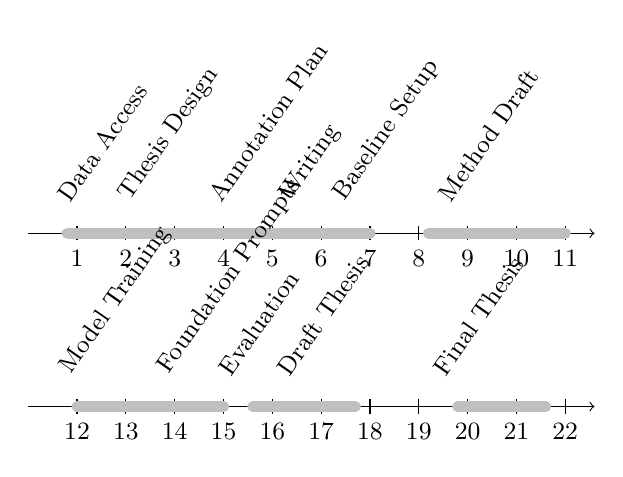
\begin{tikzpicture}[x=0.62cm,y=1cm, font=\small]

% ===== Top timeline: 1..11 =====
\draw[->] (0,0) -- (11.6,0);
\foreach \x in {1,...,11} {
  \draw (\x,0.09) -- (\x,-0.09);
  \node[below] at (\x,-0.09) {\x};
}
\node[rotate=55, anchor=south west] at (0.9,0.20) {Data Access};
\node[rotate=55, anchor=south west] at (2.2,0.20) {Thesis Design};
\node[rotate=55, anchor=south west] at (4.0,0.20) {Annotation Plan};
\node[rotate=55, anchor=south west] at (5.5,0.20) {Writing};
\node[rotate=55, anchor=south west] at (6.6,0.20) {Baseline Setup};
\node[rotate=55, anchor=south west] at (8.7,0.20) {Method Draft};

\draw[line width=4pt, gray!50, line cap=round] (0.8,0) -- (7.0,0);
\draw[line width=4pt, gray!50, line cap=round] (8.2,0) -- (11.0,0);

% ===== Bottom timeline: 12..22 =====
\begin{scope}[yshift=-2.2cm]
\draw[->] (0,0) -- (11.6,0);
\foreach \i [evaluate=\i as \lab using int(\i+11)] in {1,...,11} {
  \draw (\i,0.09) -- (\i,-0.09);
  \node[below] at (\i,-0.09) {\lab};
}
\node[rotate=55, anchor=south west] at (1.0,0.20) {Model Training};
\node[rotate=55, anchor=south west] at (3.0,0.20) {Foundation Prompts};
\node[rotate=55, anchor=south west] at (4.2,0.20) {Evaluation};
\node[rotate=55, anchor=south west] at (5.4,0.20) {Draft Thesis};
\node[rotate=55, anchor=south west] at (8.6,0.20) {Final Thesis};

\draw[line width=4pt, gray!50, line cap=round] (1.0,0) -- (4.0,0);
\draw[line width=4pt, gray!50, line cap=round] (4.6,0) -- (6.7,0);
\draw[line width=4pt, gray!50, line cap=round] (8.8,0) -- (10.6,0);
\end{scope}

\end{tikzpicture}
\caption{Project timeline overview (split across two lines to fit the page).}
\label{fig:timeline_split}
\end{figure}

\subsection{Official Milestones (UvA Deadlines)}
\begin{itemize}
    \item \textbf{Before 10 Jan:} Register project on Datanose.
    \item \textbf{23 Feb (Canvas):} Thesis Design submission (4 pages).
    \item \textbf{Before 9 Mar (Datanose):} Supervisor-approved Thesis Design.
    \item \textbf{23 Mar (Canvas):} Exploratory milestone (Literature + Dataset Plan).
    \item \textbf{20 Apr (Canvas):} Draft Methodology Section.
    \item \textbf{19 May:} Midterm Evaluation.
    \item \textbf{25 May (Canvas):} Pre-Draft Thesis (including initial Results).
    \item \textbf{15 Jun (Canvas):} Draft Thesis.
    \item \textbf{26 Jun (Datanose):} Final Thesis.
\end{itemize}

\subsection{Roadmap (Sprint-Level Plan)}
Each sprint concludes with a concrete deliverable and review checkpoint.

\begin{center}
\small
\begin{tabular}{p{0.48\linewidth} p{0.48\linewidth}}

\textbf{Sprint 1 (Jan 5--18):} Refine RQ; finalize scope; register Datanose. &
\textbf{Sprint 2 (Jan 19--Feb 1):} Thesis Design iteration; justify YOLO vs foundation models. \\

\textbf{Sprint 3 (Feb 2--15):} Finalize Thesis Design draft; prepare submission. &
\textbf{Sprint 4 (Feb 16--Mar 1):} Submit Thesis Design; define annotation schema. \\

\textbf{Sprint 5 (Mar 2--15):} Manual data annotation; dataset split definition. &
\textbf{Sprint 6 (Mar 16--29):} Submit March milestone; finalize baseline method. \\

\textbf{Sprint 7 (Mar 30--Apr 12):} Draft Methodology; define metrics and protocol. &
\textbf{Sprint 8 (Apr 13--Apr 26):} Submit Methodology; implement YOLO training pipeline. \\

\textbf{Sprint 9 (Apr 27--May 10):} Train and tune YOLO model. &
\textbf{Sprint 10 (May 11--May 24):} Prompt and instruction template design for LLaVA; foundation-model prompting (LLaVA); structured output extraction; Midterm (19 May). \\

\textbf{Sprint 11 (May 25--Jun 7):} Quantitative comparison; robustness testing; Pre-Draft (25 May). &
\textbf{Sprint 12 (Jun 8--Jun 21):} Draft Thesis (15 Jun); integrate results and discussion. \\
\textbf{Sprint 13 (Jun 22--Jun 30):} Final revisions; formatting; Final Thesis submission (26 Jun) + buffer.\\

\end{tabular}
\end{center} 
